\chapter[Exemples de Mise en Forme: Guide des Éléments LaTeX]{Exemples de Mise en Forme Guide des Éléments LaTeX}
\label{cp:examples}

Ce chapitre présente des exemples de tous les éléments de mise en forme disponibles dans ce modèle LaTeX. Vous pouvez utiliser ce chapitre comme référence pour voir comment chaque élément apparaît dans le document final.

\section{Titres et Sections}
Les sections permettent d'organiser votre document de manière hiérarchique.

\subsection{Sous-section}
Ceci est un exemple de sous-section. Les sous-sections sont utilisées pour diviser une section en parties plus petites.

\subsubsection{Sous-sous-section}
Ceci est un exemple de sous-sous-section, le niveau le plus bas de la hiérarchie des titres.

\section{Texte et Mise en Forme}

\subsection{Styles de Texte}
Voici différents styles de texte disponibles:

\begin{itemize}
    \item \textbf{Texte en gras} -- utiliser \verb|\textbf{}|
    \item \textit{Texte en italique} -- utiliser \verb|\textit{}|
    \item \underline{Texte souligné} -- utiliser \verb|\underline{}|
    \item \texttt{Texte monospace} -- utiliser \verb|\texttt{}|
    \item \textsc{Petites Capitales} -- utiliser \verb|\textsc{}|
\end{itemize}

\subsection{Citations et Blocs}

\begin{block}[note]
Ceci est un bloc de note. Il est utilisé pour mettre en évidence des informations importantes que le lecteur devrait remarquer.
\end{block}

\begin{block}[tip]
Ceci est un bloc de conseil. Il fournit des astuces utiles ou des bonnes pratiques.
\end{block}

\section{Listes}

\subsection{Liste à Puces}
\begin{itemize}
    \item Premier élément de la liste
    \item Deuxième élément de la liste
    \item Troisième élément de la liste
    \begin{itemize}
        \item Sous-élément A
        \item Sous-élément B
    \end{itemize}
\end{itemize}

\subsection{Liste Numérotée}
\begin{enumerate}
    \item Premier élément numéroté
    \item Deuxième élément numéroté
    \item Troisième élément numéroté
    \begin{enumerate}
        \item Sous-élément numéroté
        \item Autre sous-élément
    \end{enumerate}
\end{enumerate}

\subsection{Liste de Description}
\begin{description}
    \item[AI] Intelligence Artificielle -- technologie permettant aux machines d'apprendre.
    \item[Q-Checker] Outil de vérification de qualité géométrique.
    \item[CAO] Conception Assistée par Ordinateur.
\end{description}

\section{Tableaux}

\subsection{Tableau Simple}
\begin{table}[!htpb]
    \caption{Exemple de tableau simple avec l'environnement tabular.}
    \label{tab:exemple-simple}
    \centering
    \begin{tabular}{llc}
        \toprule
        \textbf{Paramètre} & \textbf{Description} & \textbf{Valeur} \\ 
        \midrule
        Épaisseur          & Épaisseur de la pièce    & 2.5 mm  \\
        Rayon              & Rayon de courbure        & 10 mm   \\
        Tolérance          & Tolérance géométrique    & 0.1 mm  \\
        \bottomrule
    \end{tabular}
\end{table}

\subsection{Tableau avec Colonnes Étendues}
\begin{table}[!htpb]
    \caption{Exemple de tableau avec l'environnement tabularx.}
    \label{tab:exemple-tabularx}
    \begin{tabularx}{\textwidth}{lX}
        \toprule
        \textbf{Composant} & \textbf{Description} \\ 
        \midrule
        Module AI & Ce module utilise des algorithmes d'apprentissage automatique pour analyser et optimiser la géométrie des pièces. \\
        Q-Checker & Outil de vérification qui valide la conformité géométrique des pièces selon les normes industrielles. \\
        Interface & Interface utilisateur permettant la visualisation et l'interaction avec les résultats d'optimisation. \\
        \bottomrule
    \end{tabularx}
\end{table}

\subsection{Tableau Complexe}
\begin{table}[!htpb]
    \caption{Exemple de tableau complexe avec multi-lignes.}
    \label{tab:exemple-complexe}
    \centering
    \begin{tabular}{lcc}
        \toprule
        \multirow{2}{*}{\textbf{Module}} & \multicolumn{2}{c}{\textbf{Caractéristiques}} \\
        \cmidrule(lr){2-3}
        & \textbf{Fonctionnalité} & \textbf{Actif} \\
        \midrule
        \multirow{3}{*}{Analyse} & Détection des défauts & $\checkmark$ \\
        & Mesure automatique & $\checkmark$ \\
        & Rapport PDF & $\checkmark$ \\
        \midrule
        \multirow{3}{*}{Optimisation} & Suggestion de corrections & $\checkmark$ \\
        & Apprentissage adaptatif & $\checkmark$ \\
        & Export CAO & - \\
        \bottomrule
    \end{tabular}
\end{table}

\section{Figures}

\begin{figure}[!htpb]
    \centering
    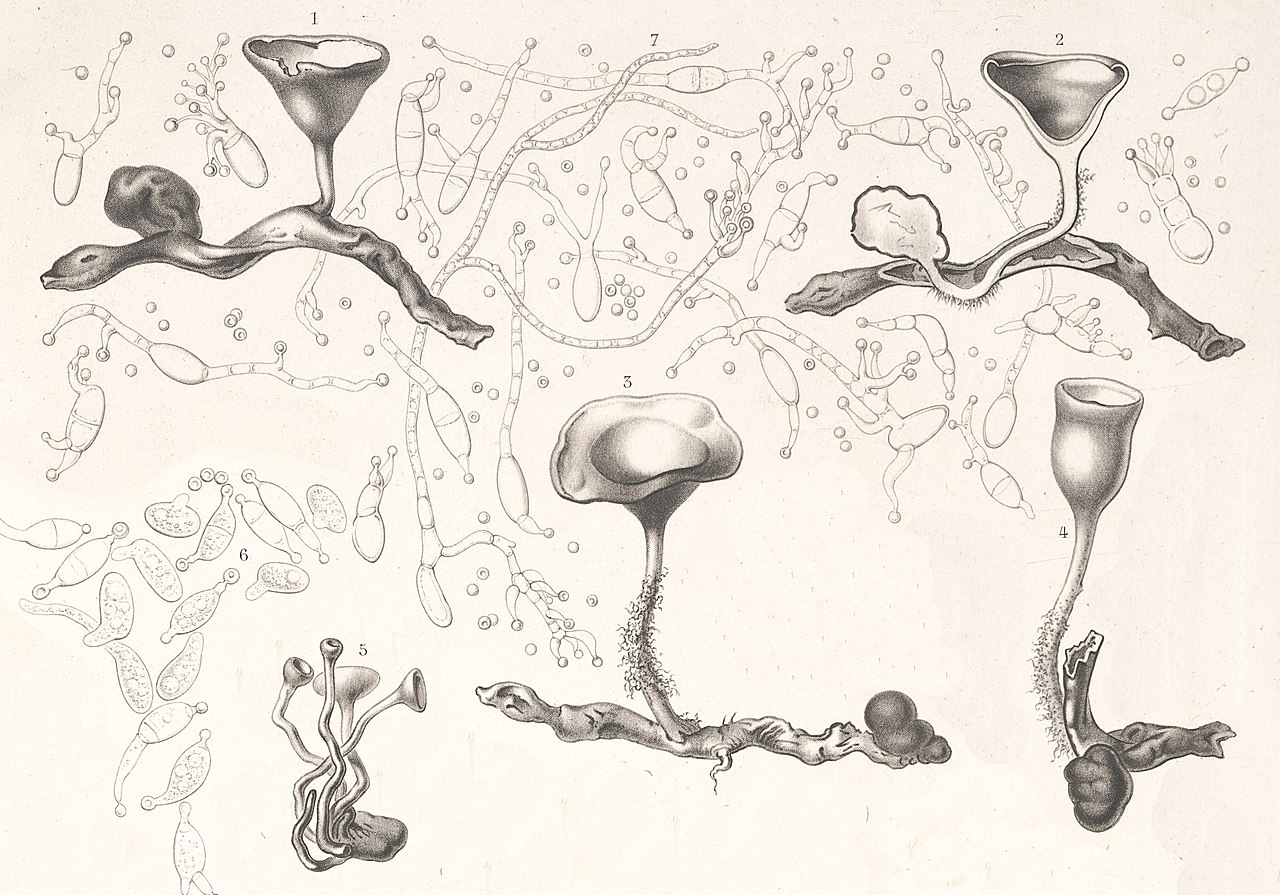
\includegraphics[width=0.7\linewidth]{Figures/PezizaTuberosa.jpg}
    \caption[Exemple de figure simple]{Exemple de figure simple. Remplacez cette image par vos propres figures pour illustrer votre travail.}
    \label{fig:exemple-figure}
\end{figure}

\section{Code Source}

\subsection{Code Inline}
Utilisez \verb|\verb| pour du code en ligne, par exemple: \verb|print("Hello World")|.

\subsection{Bloc de Code}
\begin{listing}[!htpb]
\caption{Exemple de code Python pour l'optimisation.}
\label{listing:python-exemple}
\begin{minted}{python}
import numpy as np

def optimize_geometry(parameters):
    """
    Fonction d'optimisation de géométrie.
    
    Args:
        parameters: Dictionnaire des paramètres géométriques
    
    Returns:
        Paramètres optimisés
    """
    # Algorithme d'optimisation
    optimized = {}
    for key, value in parameters.items():
        optimized[key] = value * 0.95  # Réduction de 5%
    
    return optimized

# Exemple d'utilisation
params = {"thickness": 2.5, "radius": 10.0}
result = optimize_geometry(params)
print(f"Résultat: {result}")
\end{minted}
\end{listing}

\subsection{Code depuis Fichier Externe}
\begin{listing}[!htpb]
\caption{Exemple de code Haskell importé depuis un fichier externe.}
\label{listing:haskell-exemple}
\inputminted{haskell}{Code/Factorial.hs}
\end{listing}

\subsection{Bloc Verbatim}
Pour afficher du texte brut sans mise en forme:

\begin{verbatim}
Ceci est un bloc verbatim.
Le texte est affiché tel quel,
sans aucune interprétation LaTeX.
\end{verbatim}

\section{Équations Mathématiques}

\subsection{Équation Inline}
La formule de la distance euclidienne est \(d = \sqrt{(x_2-x_1)^2 + (y_2-y_1)^2}\).

\subsection{Équation Numérotée}
\begin{equation}
\label{eq:optimization}
\min_{x} f(x) = \sum_{i=1}^{n} w_i \cdot (x_i - x_i^*)^2
\end{equation}

L'équation \ref{eq:optimization} représente une fonction objectif typique pour l'optimisation géométrique.

\subsection{Équation Sans Numéro}
\[
\mathcal{L}(\theta) = -\frac{1}{N} \sum_{i=1}^{N} \log P(y_i | x_i; \theta)
\]

\section{Références et Citations}

\subsection{Références Croisées}
Vous pouvez référencer des éléments du document:
\begin{itemize}
    \item Référence à un chapitre: \autoref{cp:examples}
    \item Référence à une section: \autoref{tab:exemple-simple}
    \item Référence à une figure: \autoref{fig:exemple-figure}
    \item Référence à une équation: Équation \ref{eq:optimization}
    \item Référence à un listing: \autoref{listing:python-exemple}
\end{itemize}

\subsection{Citations Bibliographiques}
Exemple de citation dans le texte: selon \citet{Elgamal1985}, les systèmes cryptographiques... 

Exemple de citation entre parenthèses: les méthodes de chiffrement modernes \citep{Elgamal1985}.

\section{Notes de Bas de Page}
Les notes de bas de page permettent d'ajouter des informations complémentaires\footnote{Ceci est un exemple de note de bas de page. Elle apparaît en bas de la page.}.

\section{Blocs Spéciaux}

\begin{block}[note]
\textbf{Note importante:} Ce modèle est conçu pour être flexible et s'adapter à différents types de documents académiques.
\end{block}

\begin{block}[tip]
\textbf{Conseil:} N'hésitez pas à consulter la documentation LaTeX pour découvrir d'autres fonctionnalités avancées.
\end{block}
